% HEADER
\documentclass[12pt]{article}
\usepackage{00_Preamble/frr_preamble}

% Functions/Settings
\setcounter{secnumdepth}{4}
\renewcommand{\familydefault}{cmr}
\definecolor{amber}{rgb}{1.0, 0.75, 0.0}
\setlength{\parindent}{1cm} % Default is 15pt.


% Packages
\usepackage{titlesec}	
\usepackage{hyperref}
\usepackage{float}
\usepackage{graphics}
\usepackage{placeins}
\usepackage{adjustbox}
\usepackage{array}
\usepackage{makecell}
\usepackage{graphicx}
\usepackage{sidecap}
% END HEADER


\begin{document}\thispagestyle{empty}

	% TITLE PAGE
	\documentclass[12pt]{article}
\usepackage{00_Preamble/frr_preamble}
\usepackage{tikz}

\begin{document}


	\begin{titlepage}

\setlength{\parindent}{0cm}
\newcommand{\HRule}{\rule{\linewidth}{0.25mm}}

\vspace*{0.5in}
\centering{
\huge\textsc{{Vanderbilt University}} \\

\vspace*{0.125in}

\large \textsc{2301 Vanderbilt Pl Nashville, TN 37235}
}

\vspace*{.125in}

\HRule \\[0.4cm]
%\centering{
	\Large\textsc{Vanderbilt University Robotics \\ Systems Engineering Report}

\HRule\\ [1.0cm]

\vspace*{0.0in}
\huge\textsc{NASA Robotic Mining Competition}

\vspace*{0.125in}

\LARGE{\textsc{2017 - 2018}}

\vspace*{0.2in}

\large{\textsc{April 10, 2018}}

\vspace*{0.1in}

\begin{center}
\rule{4.5in}{0.4pt}
\end{center}
\begin{center}
Dr. Nabil Simaan: Faculty Advisor \\
\end{center}

\vspace*{0.2in}
%\textbf{\underline{Executive Members:}}

\centering
\small{
 \begin{tabular}{r l r l}
  \textbf{Lin Liu ---} & President  &  \textbf{Danny Levy ---} & Vice President \\
  \textbf{Swapnil Pande ---} & Team Captain  & \textbf{Alexander Barnett ---} & Public Relations Chair \\
  \textbf{Alade Malik ---} & Secretary & \textbf{Jeffanie Wu ---} & Treasurer \\
  \textbf{Jacob Fine ---} & Design Team Lead & \textbf{Joshua Petrin ---} & Electrical Team Lead \\
  \textbf{Joseph Holliday ---} & Programming Team Lead & &
 \end{tabular}
}

\vspace*{0.2in}

\centering
\footnotesize{
 \begin{tabular}{l l l}
  \textbf{Design Team:}&  \textbf{Electrical Team:} & \textbf{Programming Team:} \\
  Alexander Stephens   &  Daniel Dong      &  Arjun Keerthi  \\
  Kimberly Majumder    &  Joshua Berger    &  Kevin Zhai     \\
  Samantha Majumder    &  Lawrence Kwok    &  Zhanwhen Chen  \\
  Stephanie Schroth    &  Minh Vu          &                 \\
  Brian Rider          &  Robert Saskowski &                 \\
  Diandry  Rutayisire  &  Rodman Zhu       &                 \\
  Emmet Hayden         &  Tristan Irvin    &                 \\
 \end{tabular}
}

\vspace*{0.3in}

\begin{tikzpicture}[remember picture,overlay]
   \node[anchor=north east,inner sep=0pt] at (current page.north east)
              {
\includegraphics[scale=0.7]{09_Figures/NASA}};
\end{tikzpicture}

\begin{tikzpicture}[remember picture,overlay]
   \node[anchor=south west,inner sep=0pt] at (current page.south west)
              {
\includegraphics[scale=0.9]{09_Figures/VUlogo3}};
\end{tikzpicture}

%}

\end{titlepage}

\end{document}

	\pagebreak
	
	% TABLE OF CONTENTS
	\phantomsection{}
	\addcontentsline{toc}{section}{Table of Contents}
	\tableofcontents\label{toc}
	\pagebreak

	% HEADER
\documentclass[class=article, crop=false]{standalone}
\usepackage{00_Preamble/frr_preamble}

% Packages
\usepackage{titlesec}	
\usepackage{hyperref}
\usepackage{float}
\usepackage{graphics}
\usepackage{placeins}
\usepackage{adjustbox}
\usepackage[table,xcdraw]{xcolor}
% END HEADER

\begin{document}
	\section{Introduction}
		% HEADER
\documentclass[class=article, crop=false]{standalone}
\usepackage{00_Preamble/frr_preamble}

% Packages
\usepackage{titlesec}
\usepackage{hyperref}
\usepackage{float}
\usepackage{graphics}
\usepackage{placeins}
\usepackage{adjustbox}
% END HEADER

\begin{document}
	\subsection{Competition Purpose}
	\label{subsec:competition_purpose}
	
	
As the Earth’s population increases and its natural resources deplete, it is essential that the world looks to the solar system for its surplus of natural resources. The aerospace industry has made huge strides towards interplanetary travel, and Mars colonization missions are now on the horizon. It is not feasible to frequently supply natural resources from Earth due to launch costs and the lead time on interplanetary travel. With the recent discovery of hydrated minerals in the Martian regolith, it is clear that In-Situ Resource Utilization (ISRU) would be essential to the development of a sustainable Mars civilization. Therefore, it is necessary to develop autonomous robotic systems for efficient water collection on Mars. The NASA Robotic Mining Competition (RMC) was established to promote the development of Mars excavation rovers and inspire the future generation of engineers to pursue ISRU technologies. Each team is tasked with designing, building, and testing a robotic excavation system in a simulated Martian environment. 
	
	
\end{document}

		
		% HEADER
\documentclass[class=article, crop=false]{standalone}
\usepackage{00_Preamble/frr_preamble}

% Packages
\usepackage{titlesec}
\usepackage{hyperref}
\usepackage{float}
\usepackage{graphics}
\usepackage{placeins}
\usepackage{adjustbox}
% END HEADER

\begin{document}
	\subsection{Problem Statement}
	\label{subsec:problem_statement}
	The robot must be capable of mining and depositing at least 1 kg of icy regolith simulant in a collector bin within 10 minutes. The mining arena consists of a 7.38 meter by 3.88 meter container with three zones: the starting zone, obstacle zone, and mining zone. The robot begins the competition run in the starting zone with an unknown orientation and must traverse the obstacle zone, mine gravel from the mining zone, and return it to the collector bin. Performance of the robot is quantified using a point system. Points are awarded and deducted based on the amount of collected gravel as well as design parameters including  the mass of the robot, energy consumption, communication bandwidth utilization, level of autonomy, and dust-free operation. 
	
	
	To simulate the limitations in the Mars environment, the robot must also adhere to certain operating limitations. The robot cannot use sound ranging systems, barometers, magnetometers, GPS, hydraulics, foam cells, or foam-filled tires, as these technologies do not work in the Martian environment. This constraint necessitates researching novel solutions to challenges which already have well-established solutions on Earth.




	
\end{document}

		
		% HEADER
\documentclass[class=article, crop=false]{standalone}
\usepackage{00_Preamble/frr_preamble}

% Packages
\usepackage{titlesec}
\usepackage{hyperref}
\usepackage{float}
\usepackage{graphics}
\usepackage{placeins}
\usepackage{adjustbox}
% END HEADER

\begin{document}
	\subsection{Purpose of Systems Engineering}
	\label{subsec:systems_engineering_purpose}
	The Vanderbilt Robotics Team followed a systems engineering design process outlined by the V-chart presented below. The excavation robot has many conflicting constraints and multiple subsystems that all need to perform equally well in order to accomplish the presented challenge. The systems engineering process provides a structured methodology to optimize competing requirements and available resources. It provides a holistic, big-picture approach to the decision making process. 
	
	\FloatBarrier
		\begin{figure}[h]
			\centering
			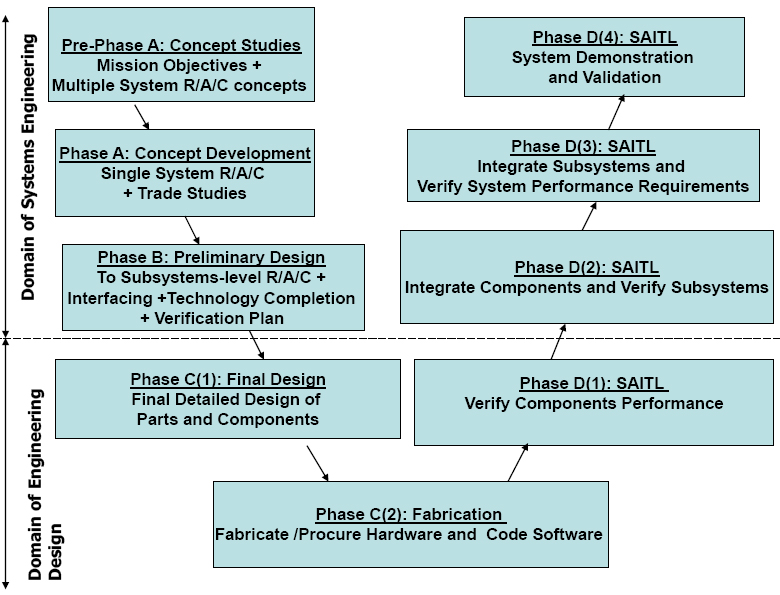
\includegraphics[width=.50\linewidth]{09_Figures/systems_engineering_vee_chart.jpg}
			\caption{Systems Engineering Vee Chart \cite{syseng}}
			\label{fig:safety_protocol_flowsheet}
		\end{figure}
		\FloatBarrier


	
\end{document}

\end{document}

	
	
	% HEADER
\documentclass[class=article, crop=false]{standalone}
\usepackage{00_Preamble/frr_preamble}

% Packages
\usepackage{titlesec}	
\usepackage{hyperref}
\usepackage{float}
\usepackage{graphics}
\usepackage{placeins}
\usepackage{adjustbox}
\usepackage[table,xcdraw]{xcolor}
% END HEADER

\begin{document}
	\section{Systems Engineering} 
		% HEADER
\documentclass[class=article, crop=false]{standalone}
\usepackage{00_Preamble/frr_preamble}

% Packages
\usepackage{titlesec}
\usepackage{hyperref}
\usepackage{float}
\usepackage{graphics}
\usepackage{placeins}
\usepackage{adjustbox}
% END HEADER

\begin{document}
	\subsection{Concept Development}
	\label{subsec:concept_development}
	\subsubsection{Design Philosophy}
	An entirely new rover design had to be developed for the team’s first year competing in the RMC. With so many design parameters, it was essential to identify a few key design considerations to focus the brainstorming and concept development process. The team focused on maximizing gravel collection, optimizing all systems for autonomy, and simplifying the fabrication process.
	
	
Optimizing gravel collection was the highest priority. The rover must excavate gravel to fulfill its main purpose. Weight and power requirements were considered as well, but it was decided to provide the weight and power necessary to reach the desired goal of excavating 40 kg of gravel. Autonomy was also essential to the design, as the success of future manned missions to Mars depends on reliable autonomous robotic aid. All systems were optimized to be fully autonomous, with the implementation of SLAM and path planning algorithms a major priority for the programming team. With only a nine month project timeline, it was important to eliminate complexity with the use of off-the-shelf components. Stock parts increase system reliability since they are manufactured to higher tolerances than possible in-house. Fabricating custom parts increases lead time and halts progress on dependent systems. However, the team decided to fabricate custom parts when needed so to not limit the design process.

	\subsubsection{System Requirements}
	The robot was designed according to the system requirements defined by NASA as well as requirements defined by Vanderbilt Robotics. The system requirements were classified by the following categories: functional, performance, and budget. All of the requirements are presented in Tables \ref{table:nasa_requirements} and  \ref{table:vur_requirements} below.
	%NASA SYSTEM REQUIREMENTS
	\FloatBarrier
	\begin{table}[h]
	\centering
	\begin{tabular}{ | m{38em} | } 
 	\hline
 		\textbf{Functional} \\ 
 		\hline
 		The robot shall fit within dimensions of 0.75 m x 1.5 m x 0.75 m at the beginning of the competition run. \\ 
 		\hline
 		The robot shall weigh no more than 80 kg. \\ 
 		\hline
 		\textbf{Performance} \\ 
 		\hline
 		The robot must be able to capable of collecting and depositing a minimum of 1 kg of icy simulant within 10 minutes. \\
 		\hline
 		The robot shall be designed to minimize dust kickup and have a dust tolerant design.  \\
 		\hline
 		The robot shall be able to function fully autonomously and failover to human control in the case of an error. \\
 		\hline
 		\textbf{Budget} \\
 		\hline
		The robot design shall be complete and verified by May 1, 2018 \\
 	\hline
	\end{tabular}
	\caption{NASA Defined System Requirements}
		\label{table:nasa_requirements}
	\end{table}
	\FloatBarrier
	
	%VUR SYSTEM REQUIREMENTS
	\FloatBarrier
	\begin{table}[h]
	\centering
	\begin{tabular}{ | m{38em} | } 
 	\hline
 		\textbf{Functional} \\ 
 		\hline
 		The robot must be capable of elevating the collected simulant a minimum of 3 inches above the collector bin. \\ 
 		\hline
 		\textbf{Performance} \\ 
 		\hline
 		The robot must be able to capable of collecting and depositing a minimum of 10 kg of icy simulant within 10 minutes. \\
 		\hline

 		\textbf{Budget} \\
 		\hline
		The project cost for development of the robot shall cost no more than \$8000. \\

 	\hline
 		
	\end{tabular}
	\caption{Vanderbilt Robotics Defined System Requirements}
		\label{table:vur_requirements}
	\end{table}
	\FloatBarrier
	
	\subsubsection{System Hierarchy}
	The system hierarchy is depicted in Figure \ref{fig:system_hierarchy}. The frame consists of the structural base of the robot, drive system, and the power distribution systems. The drivetrain was designed for direct drive. Without a suspension system, it was important to be able to control each wheel independently to maneuver obstacles and improve turning capabilities. The excavation system must dig through BP-1 and collect gravel. It was considered making these two independent processes so to not collect BP-1.  The collected gravel The robot controller software handles all input and output for the robot and maintains a state machine for higher-level control of the robot. The autonomy module includes all of the sensors for localizing the robot and mapping the environment. Additionally, all of the software associated with localization, mapping, and path planning are included in the autonomy module. The teleoperation module provides the human robot drivers with control inputs and data readouts. The autonomy module and driver station interface with the robot controller identically.
	
	\FloatBarrier
		\begin{figure}[h]
			\centering
			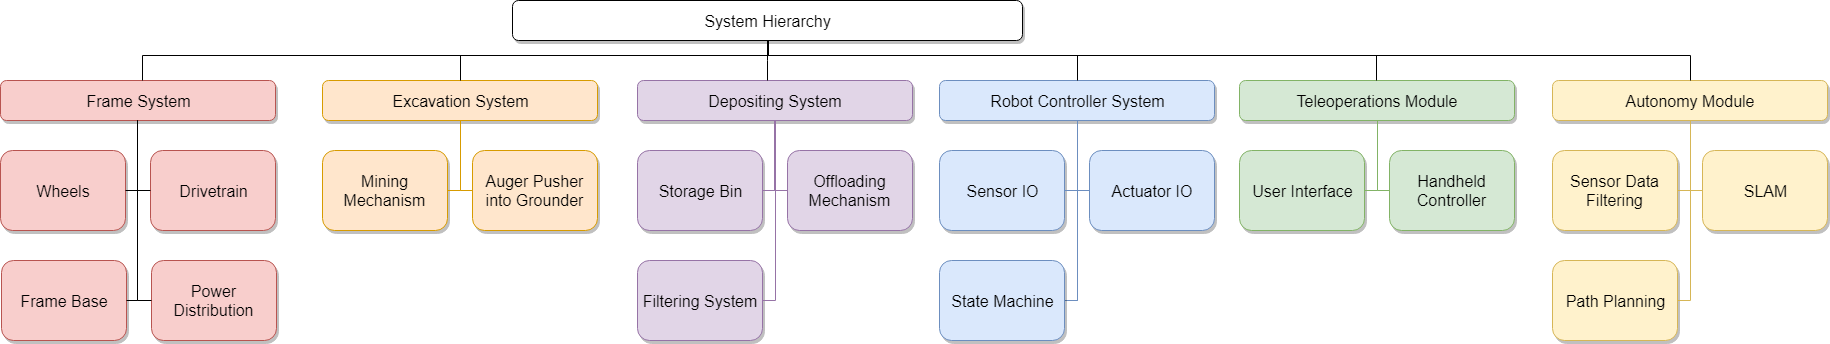
\includegraphics[width=1.0\linewidth]{09_Figures/system_hierarchy.png}
			\caption{Robot System Hierarchy}
			\label{fig:system_hierarchy}
		\end{figure}
		\FloatBarrier
		
	\subsubsection{Concept of Operations}
	The concept of operations are described in Table \ref{table:con_ops}. The order of operations was derived from the system requirements and key design considerations listed in Section 2.1.2.
	
	\ref{table:con_ops} below.
	%Concept of Operations Table
	\FloatBarrier
	\begin{table}[h]
	\centering
	\begin{tabular}{ | m{38em} | } 
 	\hline
 		\textbf{Setup} \\ 
 		\hline
 		Place robot at starting location and set up control station \\ 
 		\hline
 		Power on robot and establish network communication link \\ 
 		\hline
 		Perform calibration for sensor and control systems on the robot \\
 		\hline
 		\textbf{Competition Start} \\ 
 		\hline
 		Autonomously scan environment to determine current pose \\
 		\hline
 		Navigate to excavation zone while avoiding obstacles  \\
 		\hline
 		\textbf{Excavation} \\
 		\hline
		Mine gravel until section is depleted or storage limit is reached \\
 		\hline
 		\textbf{Post-Competition Run} \\
 		\hline
 		Record power consumption and turn off the robot \\
 		\hline
 		Clean the robot to remove particulate \\
 		\hline
 		Verify system integrity qfor next round \\
 		\hline
	\end{tabular}
	\caption{Robot Concept of Operations}
		\label{table:con_ops}
	\end{table}
	\FloatBarrier
	
	\subsubsection{System Requirements Review}
	On September 28, 2017, the executive team members met with the team’s faculty advisor and reviewed the system requirements in preparation for the preliminary design process. The system requirements were confirmed to align with the team’s design philosophy and the competition objectives...The system hierarchy was well modulated to allow for efficient task distribution and system integration. The team agreed that the concept of operations was the correct approach to satisfy both NASA’s requirements and the team-imposed autonomy and gravel collection requirements. The team received approval to proceed to the next design phase.



	
\end{document}

		% HEADER
\documentclass[class=article, crop=false]{standalone}
\usepackage{00_Preamble/frr_preamble}

% Packages
\usepackage{titlesec}
\usepackage{hyperref}
\usepackage{float}
\usepackage{graphics}
\usepackage{placeins}
\usepackage{adjustbox}
\usepackage{array}


\renewcommand{\arraystretch}{1.4}
% END HEADER

\begin{document}
	\subsection{Preliminary Design}
	\label{subsec:preliminary_design}
	Each system on the robot went through multiple design iterations during the preliminary design process. Significant background research was conducted into the Mars environment, potential excavation systems, drivetrain, and path planning and SLAM implementations. Trade studies were combined with testing to determine the best and most realistic rover design.
	\subsubsection{Drive System}
In order to determine the behavior of drive systems in the competition conditions, research was conducted on drive systems used by various teams from previous years. Many robots encountered wheel slippage and struggled to maneuver out of steep ditches. In order to achieve the goal of autonomy, the team aimed to design the drive system to minimize slippage and maximize maneuverability.

Two potential drive mechanisms were considered: a 4-wheel direct drive and tank tread drive. A trade study for the drive systems considered is shown in Table \ref{table:drive_trade_study}. The tank tread drive is superior to the wheeled drive system in traction and obstacle traversal. However, due to the increased number of parts, it is also less power efficient, heavier, and more difficult to manufacture. The 4-wheel direct drive has very few moving components, making system integration and assembly much simpler. However, few off-the-shelf wheels exist that satisfy the design parameters, necessitating the wheels to be custom-manufactured. While a wheeled drive does not have as much traction as the tank tread drive, independent control for all four wheels allows for advanced control algorithms to monitor and correct wheel slippage. Additionally, the system would be fail-operational in the case a of single drive motor failure. Due to the simpler design implementation and independent control of each wheel, the four wheel direct drive system was selected.



\FloatBarrier
	\begin{table}[h]
	\footnotesize
	\centering
	\begin{tabular}{ | p{8em} | m{4em} | m{6em} | m{3em} | m{8em} | m{3em} | }
 	\hline
 		\rowcolor[gray]{0.8}
 		\textbf{Factor} &\textbf{Weight} &\textbf{Tank Tread Drive} &\textbf{Score} &\textbf{4-Wheel Direct Drive} &\textbf{Score}  \\ 
 		\hline
		Fabrication                       &  \multicolumn{1}{c|}{0.7}  &  \multicolumn{1}{c|}{8}    &  \multicolumn{1}{c|}{5.6}  &  \multicolumn{1}{c|}{4}    &  \multicolumn{1}{c|}{2.8}   \\ 
 		\hline
 		Obstacle \mbox{Avoidance}         &  \multicolumn{1}{c|}{0.9}  &  \multicolumn{1}{c|}{7}    &  \multicolumn{1}{c|}{6.3}  &  \multicolumn{1}{c|}{9}    &  \multicolumn{1}{c|}{8.1}   \\ 
 		\hline
 		\mbox{Control System} Complexity  &  \multicolumn{1}{c|}{0.6}  &  \multicolumn{1}{c|}{9}    &  \multicolumn{1}{c|}{5.4}  &  \multicolumn{1}{c|}{6}    &  \multicolumn{1}{c|}{3.6}   \\
 		\hline
 		Power \mbox{Efficiency}           &  \multicolumn{1}{c|}{0.4}  &  \multicolumn{1}{c|}{5}    &  \multicolumn{1}{c|}{2}    &  \multicolumn{1}{c|}{9}    &  \multicolumn{1}{c|}{3.6}   \\ 
 		\hline
 		Obstacle \mbox{Traversal}         &  \multicolumn{1}{c|}{0.7}  &  \multicolumn{1}{c|}{8}    &  \multicolumn{1}{c|}{5.6}  &  \multicolumn{1}{c|}{7}    &  \multicolumn{1}{c|}{4.9}   \\
 		\hline
 		\mbox{Reliability and} Simplicity &  \multicolumn{1}{c|}{0.6}  &  \multicolumn{1}{c|}{4}    &  \multicolumn{1}{c|}{2.4}  &  \multicolumn{1}{c|}{9}    &  \multicolumn{1}{c|}{5.4}   \\
 		\hline
 		\rowcolor[gray]{0.9}
 		\textbf{Total}                    &       &       &\multicolumn{1}{c|}{\textbf{27.3}}&       &\multicolumn{1}{c|}{\textbf{28.4}}\\
 		\hline
	\end{tabular}
	\caption{Trade Study Matrix for Drive System }
		\label{table:drive_trade_study}
	\end{table}
	\FloatBarrier
	
	\subsubsection{Wheels}
	The wheels were designed to find a compromise between traction, obstacle-traversal ability, weight, and build complexity. The preliminary wheel design can be seen in Figure \ref{fig:cad-wheel-prelim}. The wheels have a 30 cm diameter to be able to climb over smaller obstacles. Based on research into rover wheel design, the team determined that grousers were required to provide traction in the loose BP-1. 12 grousers were chosen to be a good compromise between traction and a smooth ride to reduce vibration and sensor noise. The red spacers are 3D printed to fasten the grousers, wheel sides, and rim together. 6061-T6 aluminum was selected due to its low weight, relatively high strength, and machinability.
	
	\FloatBarrier
		\begin{figure}[h]
			\centering
			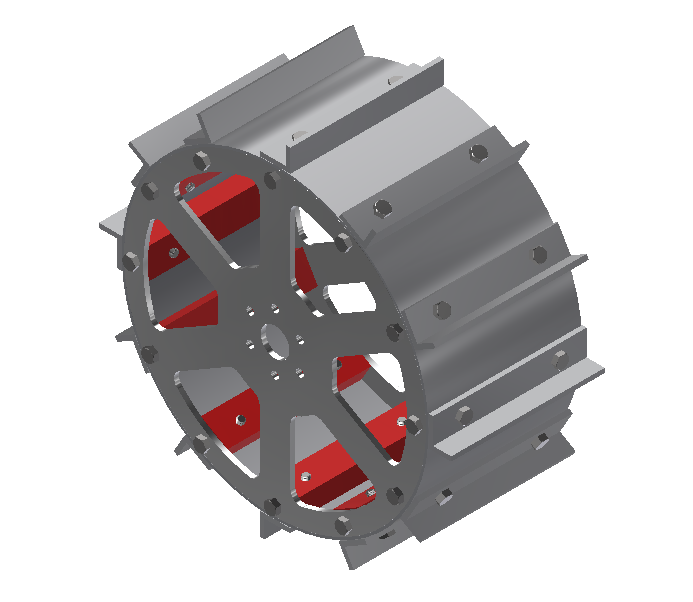
\includegraphics[width=0.4\linewidth]{09_Figures/wheel-cad-preliminary.jpg}
			\caption{CAD model of preliminary wheel design.}
			\label{fig:cad-wheel-prelim}
		\end{figure}
		\FloatBarrier

	\subsubsection{Excavation}
The main requirement for the excavation system was to dig through 30 cm of BP-1 and collect the icy regolith simulant underneath. The primary design considerations for the digging mechanism were reliability, dust tolerance, complexity, and weight. 
Research was performed on existing digging mechanisms in the mining industry. Table \ref{table:dig-trade-study} shows a trade study of potential mining mechanisms. The backhoe and bucket wheel excavator were eliminated from the solution space as they are primarily effective for surface mining. Additionally, the bucket wheel excavator is capable of removing a large amount of material, but does not fit within the size constraints of the robot.
The chain trencher, which consists of a large chain that draws material out of the ground, is capable of achieving a higher rate of gravel removal than an auger. After consulting with engineers at Ditch Witch, it was determined that a chain trencher of the correct scale for the mining robot would require at least 4 horsepower to drive. The increase in mass and energy usage for the chain trencher does not justify the increased rate of gravel collection.

The auger mechanism provides a compromise between weight, power consumption, and the mass of gravel collected. The rate of gravel collection and power consumption can be scaled by the diameter of the auger, allowing the system to be better designed for the robot. Additionally, fabrication and assembly of the auger system is significantly simpler than that for the chain trencher. Therefore, the auger was selected as the excavation mechanism.

Experiments were conducted to test the effectiveness of elevating sand and gravel through a PVC pipe using an auger. The results from the experiment demonstrated that the auger is capable of excavating gravel. Furthermore, it was found that the auger performed best at an angle of approximately 60 degrees. 



\FloatBarrier
	\begin{table}[h]
	\scriptsize
	\centering
	\begin{tabular}{ | r | c | c | c | c | c | c | c | c | c | c |}
 	\hline
 		\rowcolor[gray]{0.8}
 		\textbf{.} &\textbf{Cost} &\textbf{Fabrication} &\textbf{Power} &\makecell{\textbf{Operative} \\ \textbf{Complexity}} &\textbf{Robustness} &\makecell{\textbf{Scoring} \\ \textbf{Potential}} &\textbf{Mass} & \makecell{\textbf{Ease of} \\ \textbf{Integration}} &\textbf{Size} &  \\ 
 		\hline
		\makecell{\textbf{Decision} \\ \textbf{Weight:}}& \textbf{0.1} &\textbf{0.15} &\textbf{0.1} &\textbf{0.05} &\textbf{0.05} &\textbf{0.2} &
		\textbf{0.1} &\textbf{0.1}  &\textbf{0.15} &\makecell{\textbf{\underline{Weighted}} \\ \textbf{\underline{Score}}}  \\ 
 		\hline\hline
 		\makecell{\textbf{Auger and} \\ \textbf{Tube}}    & 8 & 8 & 7 & 8 & 6 & 3 & 6 & 5 & 7 & \textbf{6.15} \\ 
 		\hline
 		\makecell{\textbf{Chain} \\ \textbf{Trencher}}    & 6 & 8 & 1 & 9 & 7 & 10 & 2 & 3 & 2 & \textbf{5.5} \\
 		\hline
 		\makecell{\textbf{Bucket} \\ \textbf{Excavator}}  & 6 & 5 & 4 & 7 & 3 & 1 & 7 & 10 & 6 & \textbf{4.05} \\
 		\hline
 		\makecell{\textbf{Plow and} \\ \textbf{Back-hoe}} & 5 & 5 & 4 & 5 & 2 & 2 & 3 & 2 & 2 & \textbf{3.2} \\
 		\hline
 		\makecell{\textbf{Circular} \\ \textbf{Excavator}}& 5 & 2 & 6 & 8 & 3 & 6 & 2 & 7 & 1 & \textbf{4.2} \\ 
 		\hline
	\end{tabular}
	\caption{Trade Study Matrix for Digging Mechanism}
		\label{table:dig-trade-study}
	\end{table}
	\FloatBarrier
	
	
	\subsubsection{Depositing}
	Once the icy regolith is collected, it must be stored on the robot until it can be deposited in the collection bin. It was determined that it would be easiest to run the depositing system from the end of the excavation system to the back of the robot. The robot can then be driven in reverse to the collection bin and can avoid the wheel slippage that occurs when making large turns. The excavation system will extract a lot of BP-1, which does not count for points in the competition and increases power consumption due to the added weight. It was decided to use a weaved conveyor belt with a mesh aperture that allows BP-1 to fall to the ground while retaining the icy regolith.
	
	
	\subsubsection{Autonomy}
	The autonomy module is responsible for localizing the robot and providing control commands to navigate the robot around the field. Multiple sensor options for localization and obstacle avoidance were researched. 2D/3D LIDAR systems, cameras, Microsoft Kinect (Figure \ref{fig:kinect-pic}), telemetry sensors such as encoders, and inertial measurement units were all considered. These sensors were each evaluated based on performance parameters such as update rate, computational complexity, price, and noise.
	
	LIDAR based systems were considered due to their widespread use in mapping and localization tasks such as self-driving cars. LIDAR produces high-resolution depth maps of the environment and function  well in environments with limited visibility. However, many 3D LIDAR sensors, which produce a three dimensional scan of the environment, are cost-prohibitive and are not feasible within the team’s budget. While some 2D LIDAR systems fall within the budget,they only produce a planar scan of the environment. Since the obstacles on the field are low to the ground, it would be difficult to find a suitable place to mount the LIDAR system on the robot. 
	
	\begin{wrapfigure}{l}{0.5\textwidth}
	\centering
	 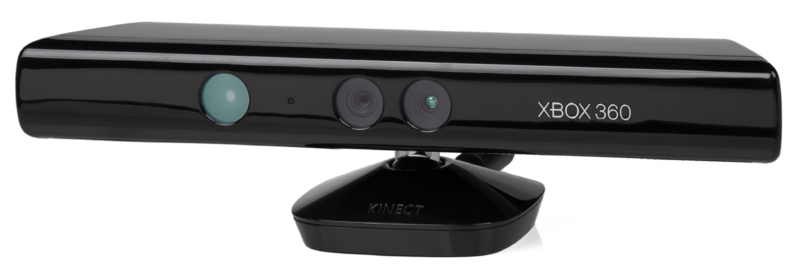
\includegraphics[width=0.48\textwidth]{09_Figures/xbox-360-kinect.png}
	 \caption{The XBox Kinect, V1}
	 \label{fig:kinect-pic}
	\end{wrapfigure}
	
	In order to localize the robot using a camera system, fiducial markers are often placed at a predefined location to serve as a landmark. The robot then determines its pose using a coordinate transformation. The OpenCV library has pre-built functions for determining robot pose by detecting AruCo markers, which are binary square fiducial markers. This method of localization is advantageous because the time required to implement is low compared to other options. However, since the camera is operating in the visual light spectrum, it may be prone to error measurement due to dust kickup. Additionally, ranging with a single camera may not be as accurate because it relies solely on the relative image size instead of time of flight measurements or stereoscopy.
	
	The Microsoft Kinect is a robust, low-cost, 3-dimensional vision system. The Microsoft Kinect outperforms LiDAR systems in dusty conditions due to its use of structured light three dimensional scanning.~\footnote{C. Hall, "Comparing the Performance Of Structured Light Depth Sensors and Traditional Time-of-flight Depth Sensors For Use in a Lunar Mining Environment", Master's, University of Alabama, 2014.} The kinect has an extensive amount of libraries for collecting and utilizing data for depth mapping and feature detection that could be adapted to match the autonomy module requirements. 
	
	An Inertial measurement unit (IMU) measures acceleration and angular velocity at a high refresh rate. However, since double integration is required to estimate position, the error accumulation rate makes the data unreliable. Instead, an IMU can be used in combination with encoder telemetry data on the drive motors to correct wheel slippage error. By comparing the acceleration and angular velocity measurements from the encoder to the expected values based the IMU data, erroneous data can be eliminated and the wheel velocities can be adjusted to correct for slippage
	
	Based on research conducted for each sensor system, it was determined that the best suited option for the robot would be a combination of a Microsoft Kinect, a camera for AruCo marker tracking, an inertial measurement unit, and encoders for telemetry data. The camera, encoders, and IMU will be used to localize the robot while the Kinect will  be used to track obstacles on the field.
	
	\subsubsection{Robot Controller}
	
	The robot controller is responsible for interpreting sensor inputs, controlling motors, and making autonomous decisions. Each of these tasks have  different hardware requirements. Sensor interpretation and motor control require a variety of IO protocols and real-time operation, whereas autonomy requires high computational power and the ability to parallelize operations (see Figure \ref{fig:data-control}). Each of these systems must also maintain low profiles to fit in a restricted space and must minimize power consumption. Multiple low-powered computers were considered:
	\begin{itemize}
	 \item Raspberry Pi provides a high level of community support and computational power, but remains limited by its IO, lack of real-time operation, and ARM architecture.
	 \item Arduinos provide a large amount of IO but provide very little computational power and difficulty interfacing with Linux based controllers.
	 \item BeagleBone Black provides similar IO to an Arduino with Linux support but lacks computational power.
	 \item BeagleBone Blue has the most IO ports and interfaces of the considered controllers. Its layout is designed for robotics applications and for interfacing with common sensors and actuators. 
	 \item The UP Board provides the best computational power whie maintaining the form factor of the Raspberry Pi, but draws substantially more power and retains the Pi’s limited IO.
	\end{itemize}
	
	The BeagleBone Blue was selected to meet the high level of connectivity required on the robot and the UP Board was selected to provide the computational power required by the autonomy module.
	
	The robot controller software must support a high level of performance, interface with open-source robotics software, and run across multiple connected controllers. However, it also must be simple enough to minimize the training time required for novice team members to begin contributing to software development.
	
	Based on these criteria, ROS (Robot Operating System) was identified as the primary software platform for the robot controller. It provides access to an extensive collection of pre-written robot libraries, greatly reducing the amount of code that needs to be written. In addition, ROS provides a network layer for running applications across a network of devices, supporting the requirement of easy communication between devices on the controller’s distributed system. 
	
	ROSMOD, an application developed by the Institute for Software Integrated Systems at Vanderbilt, allows for the development of distributed ROS applications in a graphical user interface. It simplifies code development by abstracting the hardware from the software. All software is ready to run on any device connected to it which meets the software requirements. ROSMOD helps to reduce the large amount of knowledge and boilerplate code required to properly implement distributed systems in ROS. The final decision was made to use ROSMOD to gain the full advantages of the ROS library with an easy way to develop and deploy code.

	\FloatBarrier
	\begin{figure}[h]
	\centering
	 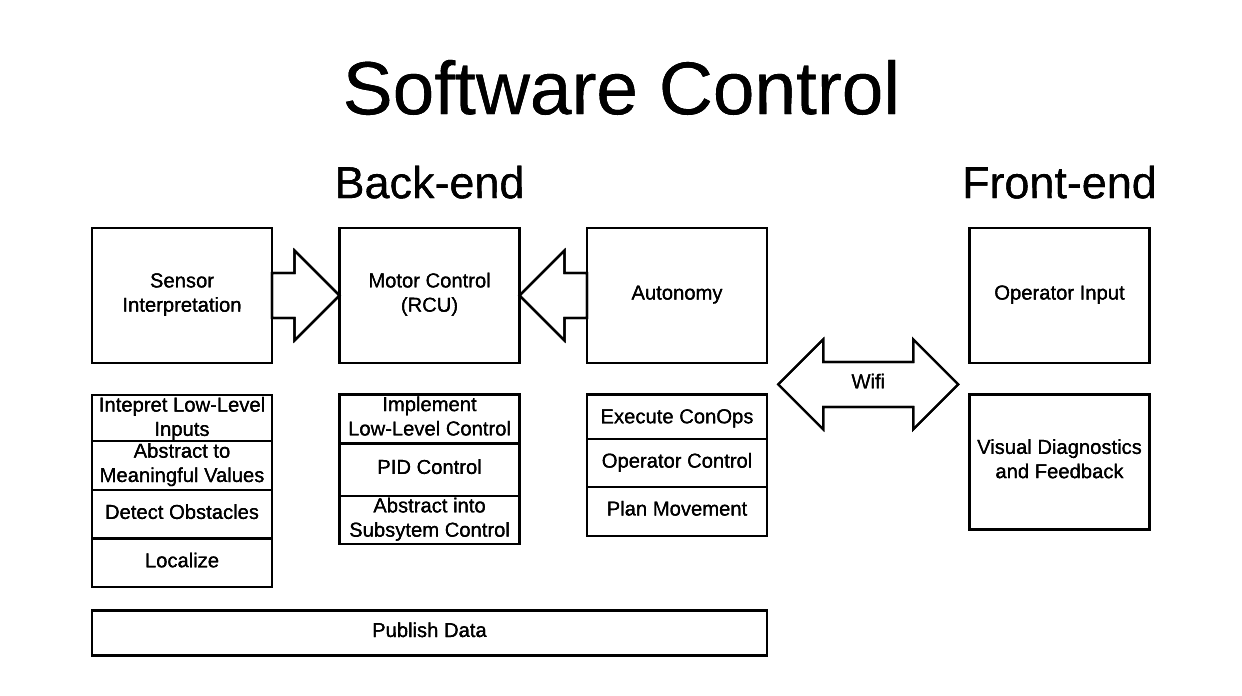
\includegraphics[width=0.8\linewidth]{09_Figures/data-control-high-level.jpg}
	 \caption{Robot Controller flow diagram}
	 \label{fig:data-control}
	\end{figure}
	\FloatBarrier
	
	
	
	\subsection{Preliminary Design Review}
	
	On January 10th, the executive team members met with the team’s faculty advisor to review the proposed preliminary designs. The preliminary design of each subsystem was verified to satisfy the design requirements. The team was cleared to move on the final design stage. 

	
	


	
\end{document}

		% HEADER
\documentclass[class=article, crop=false]{standalone}
\usepackage{00_Preamble/frr_preamble}

% Packages
\usepackage{titlesec}
\usepackage{hyperref}
\usepackage{float}
\usepackage{graphics}
\usepackage{placeins}
\usepackage{adjustbox}
% END HEADER

\begin{document}
	\subsection{System Assembly and Testing}
	\label{subsec:system_assembly_and_testing}
\end{document}

		% HEADER
\documentclass[class=article, crop=false]{standalone}
\usepackage{00_Preamble/frr_preamble}

% Packages
\usepackage{titlesec}
\usepackage{hyperref}
\usepackage{float}
\usepackage{graphics}
\usepackage{placeins}
\usepackage{adjustbox}
% END HEADER

\begin{document}
	\subsection{Project Management}
	\label{subsec:project_management}
	
	\subsubsection{Management Structure}
	Team members were distributed among three subgroups, mechanical, electrical, and programming, based on their area of interest and expertise. Members of each subteam were assigned to specific subsystems of the robot and worked in cross-disciplinary groups with other members from each subteam to fully design the subsystem. The purpose of the cross-functional groups was to ensure that all aspects of the design are considered simultaneously. Each of the subteams were managed by a subteam lead, whose responsibility was to allocate work and track progress for the design of their respective part of the robot. The subteam leads reported their progress to the team captain. The captain was responsible for tracking objectives, facilitating integration between various subteams, and ensuring that the high-level requirements are met.
	
	\subsubsection{Work Schedule}
	The team built a GANTT chart in order to track the timeline and managing deadlines for the robot design. The timeline was regularly reviewed and re-evaluated based on the progress and updated goals based on design changes. The GANTT chart is present in Appendix XX Figure XX.
	
	\subsubsection{Cost Budget}
	
	The Vanderbilt Robotics team received support from several financial sponsors this year: Vanderbilt School of Engineering, SDP/SI, Torc Robotics, Misumi, and Advanced Motion Controls. An account was established in the Vanderbilt Mechanical Engineering department to manage parts ordering. A Piggybackr crowd-sourced fundraiser account was also established to raise money from the public. The Treasurer and Public Relations Chair on the executive board were responsible for purchasing project components with the team’s financial adviser and managing the budget and the bill of materials. 
	
	An overview of the financial budget can be seen in Table \ref{table:cost_budget}. The estimated costs for the excavation, depositing, and frame and drive systems were not much less than the actual costs. The power distribution and control electronics ended up being significantly more expensive than expected, since the team did not own any electrical components at the beginning of the year. A separate travel budget was created for the competition trip. 
	
	\FloatBarrier
	\begin{table}[h]
	\scriptsize
	\centering
	\begin{tabular}{ | r | c | c | c | c | c | }
 	\hline		
 	\rowcolor[gray]{0.8}
 		\textbf{Subsystem} & \textbf{Excavation} & \textbf{Depositing} & \textbf{Frame} & \textbf{Power Distribution \& Control Electronics} & \textbf{Total} \\
 		\hline\hline
 		\textbf{Estimated Cost} & \$1,000.00 & \$500.00 & \$2,184.00 & \$800.00 &  \$4,484.01 \\
	\hline
		\textbf{Actual Cost} & \$1,662.43 & \$716.67 & \$2,618.22 & \$2,033.22 & \$7,029.54 \\
	\hline
	\end{tabular}
	\caption{Cost Budget Allocation Summary}
		\label{table:cost_budget}
	\end{table}
	\FloatBarrier
\end{document}

		% HEADER
\documentclass[class=article, crop=false]{standalone}
\usepackage{00_Preamble/frr_preamble}

% Packages
\usepackage{titlesec}
\usepackage{hyperref}
\usepackage{float}
\usepackage{graphics}
\usepackage{placeins}
\usepackage{adjustbox}
% END HEADER

\begin{document}
	\subsection{Technical Management}
	\label{subsec:technical_management}
	
\end{document}

		

\end{document}

	\pagebreak
	
	% HEADER
\documentclass[class=article, crop=false]{standalone}
\usepackage{00_Preamble/frr_preamble}

% Packages
\usepackage{titlesec}	
\usepackage{hyperref}
\usepackage{float}
\usepackage{graphics}
\usepackage{placeins}
\usepackage{adjustbox}
\usepackage[table,xcdraw]{xcolor}
% END HEADER

\begin{document}
	\section{Conclusions}
		The Vanderbilt Robotics Team has used a systems engineering approach to design an autonomous Mars excavation rover for the 2018 NASA RMC. The rover design seeks to find an elegant solution to the complex challenge of natural resource mining on Mars and help develop the autonomous space robotics field, since it is essential to the future of interplanetary travel. 
		
		The final robot design had many strong points, such as its ease of assembly and custom fabricated systems. With the experience and prototypes developed this year, the team will continue to optimize the robot design in attributes such as weight, power efficiency, and autonomy in future years.


\end{document}

	
<<<<<<< HEAD
	\pagebreak
	
=======
>>>>>>> appendix-a
	% HEADER
\documentclass[class=article, crop=false]{standalone}
\usepackage{00_Preamble/frr_preamble}

% Packages
\usepackage{titlesec}	
\usepackage{hyperref}
\usepackage{float}
\usepackage{graphics}
\usepackage{placeins}
\usepackage{adjustbox}
\usepackage[table,xcdraw]{xcolor}
% END HEADER

\begin{document}
\renewcommand\refname{Bibliography}
	\begin{thebibliography}{9}
	
	\end{thebibliography}
\end{document}


	\addcontentsline{toc}{section}{Bibliography}
	
	% HEADER
\documentclass[class=article, crop=false]{standalone}
\usepackage{00_Preamble/frr_preamble}

% Packages
\usepackage{titlesec}	
\usepackage{hyperref}
\usepackage{float}
\usepackage{graphics}
\usepackage{placeins}
\usepackage{adjustbox}
\usepackage[table,xcdraw]{xcolor}
% END HEADER

\begin{document}
 
\newpage
\section{Appendix A}

\noindent
\Large Below are defined the requirements for all subsystems on the Vanderbilt University Robotics robot: \vspace*{0.1in}


\noindent
\normalsize
Frame:
\footnotesize

\vspace*{0.05in}
\noindent
\emph{Functional}
\begin{itemize}
 \item Must be able to successfully traverse Martian terrain
 \item Must support the excavation and deposit systems
 \item Must contain the drivetrain
 \item Must fit within competition size constraints at the beginning of the competition run
\end{itemize}
\noindent
\emph{Performance}
\begin{itemize}
 \item Must have minimal wheel slippage
 \item Must be able to be controlled autonomously
 \item Must be lightweight
\end{itemize}
\noindent
\emph{Budget}
\begin{itemize}
 \item Must cost less than \$2,000
\end{itemize}
\vspace*{0.1in}


\noindent
\normalsize
Excavation:
\footnotesize

\vspace*{0.05in}
\noindent
\emph{Functional}
\begin{itemize}
 \item Must dig through 30 cm of BP-1
 \item Must excavate icy regolith 
 \item Must deposit icy regolith into the deposit system
\end{itemize}
\noindent
\emph{Performance}
\begin{itemize}
 \item Must excavate a minimum of 10 kg of icy regolith
\end{itemize}
\noindent
\emph{Budget}
\begin{itemize}
 \item Must cost less than \$1,000
\end{itemize}

\vspace*{0.1in}

\noindent
\normalsize 
Depositing:
\footnotesize

\vspace*{0.05in}
\noindent
\emph{Functional}
\begin{itemize}
 \item Must store icy regolith during competition round
 \item Must deposit icy regolith in collection bin
\end{itemize}
\noindent
\emph{Performance}
\begin{itemize}
 \item Must be able to store at least 50 kg of icy regolith
 \item Must carry icy regolith to a height of 3 in. above the collection bin
\end{itemize}
\noindent
\emph{Budget}
\begin{itemize}
 \item Must cost less than \$500
\end{itemize}

\vspace*{0.1in}

\noindent
\normalsize 
Power Distribution:
\footnotesize

\vspace*{0.05in}
\noindent
\emph{Functional}
\begin{itemize}
 \item All electronic devices on the robot must be powered at their nominal voltage (but not necessarily be on at all times during the competition)
 \item The entire electrical system must be regulated by a red emergency shutoff switch
 \item The batteries must satisfy the aggregate capacity requirements of all electrical subsystems
\end{itemize}
\noindent
\emph{Performance}
\begin{itemize}
 \item Each electrical component on the robot must have at least a 20\% safety factor in each current-capacity aspect
\end{itemize}
\noindent
\emph{Budget}
\begin{itemize}
 \item Only one battery configuration can be used
\end{itemize}

\vspace*{0.1in}

\noindent
\normalsize
Robot Controller:
\footnotesize

\vspace*{0.05in}
\noindent
\emph{Functional}
\begin{itemize}
 \item Must be capable of actuating every motor on the robot
 \item Must interface with every sensors (directly or indirectly) on the robot
\end{itemize}
\emph{Performance}
\begin{itemize}
 \item Must utilize as little network bandwidth as possible
\end{itemize}
\noindent
\emph{Budget}
\begin{itemize}
 \item Must cost no monetary value
\end{itemize}

\vspace*{0.1in}

\noindent
\normalsize
Autonomy:
\footnotesize
\vspace*{0.05in}

\noindent
\emph{Functional}
\begin{itemize}
 \item The autonomy module shall be capable of localizing the robot from an unknown starting position
 \item The autonomy module shall be able to detect and avoid obstacles such as boulders and ditches
 \item The autonomy module shall communicate with the robot controller with standard control commands
\end{itemize}

\noindent
\emph{Perfomance}
\begin{itemize}
 \item The autonomy module shall be capable of navigating the robot back and forth from the starting zone to the mining zone
 \item The autonomy module shall be able to detect failover to human control in case of an error mode
\end{itemize}

\noindent
\emph{Budget}
\begin{itemize}
 \item The autonomy module shall have as little computation requirements as possible
\end{itemize}

\end{document}

	
	% HEADER
\documentclass[class=article, crop=false]{standalone}
\usepackage{00_Preamble/frr_preamble}

% Packages
\usepackage{titlesec}	
\usepackage{hyperref}
\usepackage{float}
\usepackage{graphics}
\usepackage{placeins}
\usepackage{adjustbox}
\usepackage[table,xcdraw]{xcolor}
% END HEADER

\begin{document}
	\section{Appendix B - Gantt Chart}
	
	\FloatBarrier
		\begin{figure}[h]
			\centering
			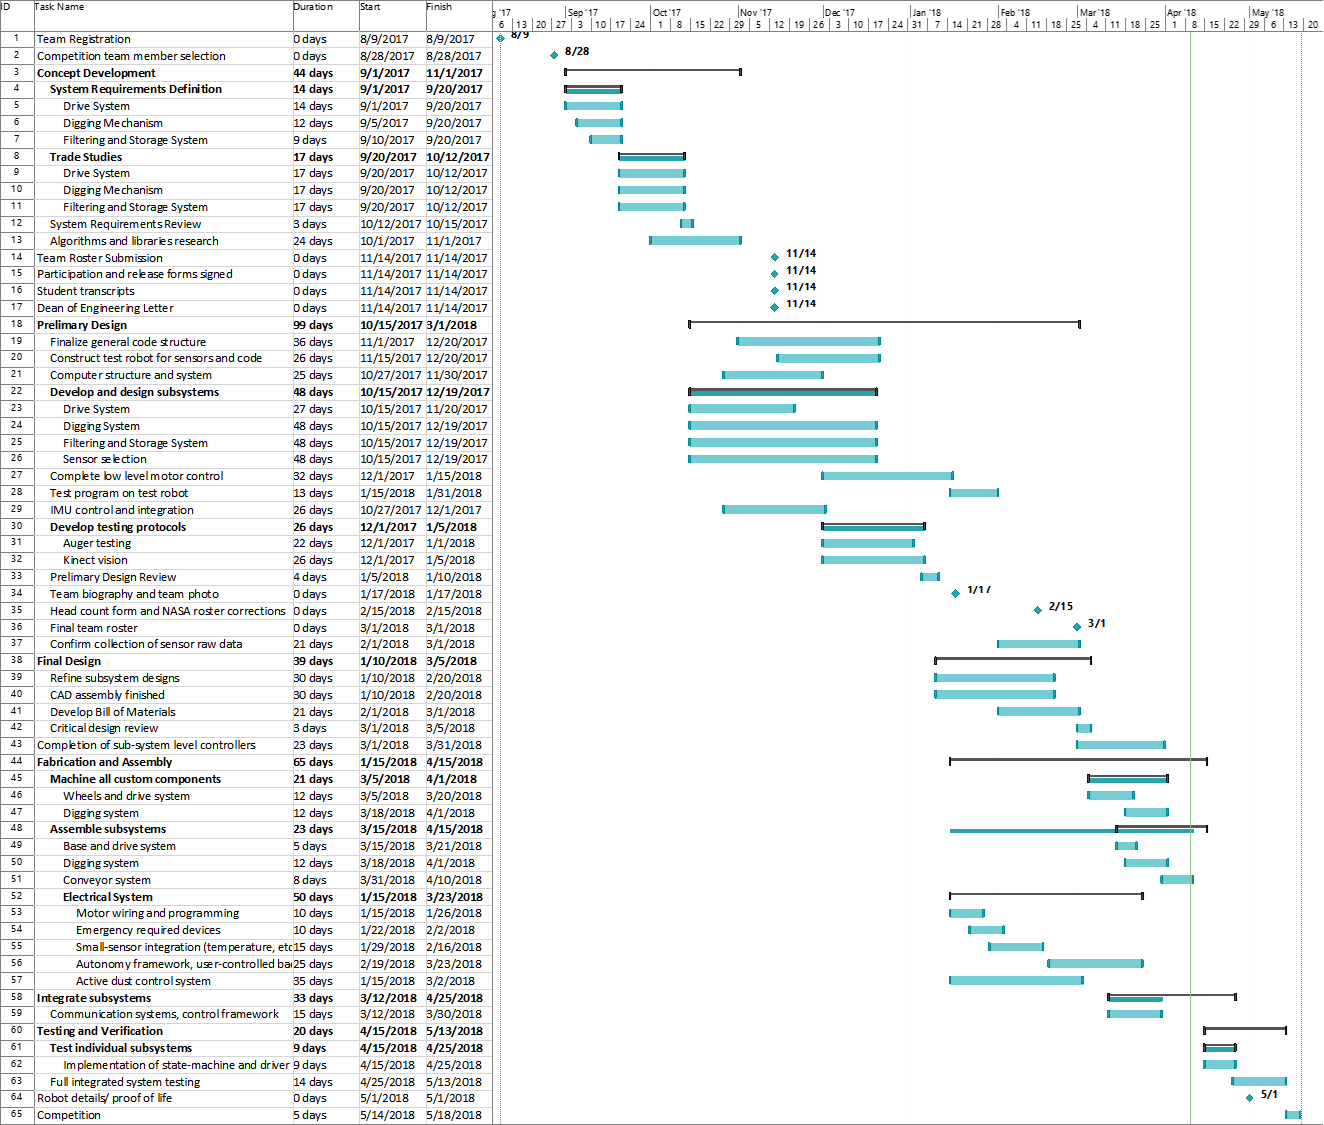
\includegraphics[width=1\linewidth]{09_Figures/gantt_chart.png}
			\caption{Robot System Hierarchy}
			\label{fig:gantt_chart}
		\end{figure}
		\FloatBarrier	
	
\end{document}

	
	\pagebreak

  \end{document}
